\documentclass[conference]{IEEEtran}
\IEEEoverridecommandlockouts
\usepackage{cite}
\usepackage{amsmath,amssymb,amsfonts}
\usepackage{algorithmic}
\usepackage{graphicx, caption, subcaption}
\usepackage{circuitikz}
\usepackage{textcomp}
\usepackage{xcolor}
\usepackage{siunitx}
\sisetup{
  range-phrase = --,      % use en-dash for ranges
  range-units = single    % place unit only at the end
}
\usepackage{hyperref}
\usepackage{upgreek}
\def\BibTeX{\rm B\kern-.05em{\sc i\kern-.025em b}\kern-.08em
    T\kern-.1667em\lower.7ex\hbox{E}\kern-.125emX}

\begin{document}

\title{Development and Characterization of a Gold-Bump Flip-Chip Bonding Process for RF IC Applications
}

\author{\IEEEauthorblockN{Daniel Tyukov, Timo Matray, Marco Fattori, Vojkan Vidojkovic, Georgi Radulov}
\IEEEauthorblockA{Integrated Circuits Group, Department of Electrical Engineering\\
Eindhoven University of Technology\\
Eindhoven, The Netherlands\\
d.tyukov@student.tue.nl; \{t.m.matray, m.fattori, v.vidojkovic, g.radulov\}@tue.nl}}

\maketitle

\begin{abstract}
Gold bump flip-chip interposers on glass offer the low-parasitic interconnects required for next-generation RF system-in-package (SiP) assemblies. Existing approaches often rely on multilayer metal stacks and complex bonding profiles. This work presents a simplified alternative: a single-layer Ti/Au ground-signal-ground coplanar waveguide interposer, bonded to a GaN chip using \SI{70}{\micro\meter} thermosonically placed gold bumps. The process encompasses bump formation, flip-chip thermo-compression, and open-short de-embedding. Broadband electrical measurements are reduced to a lumped-element bump model, which can be directly integrated into a process design kit, enabling cost-effective RF SiP prototyping on glass substrates.
\end{abstract}

\begin{IEEEkeywords}
flip-chip bonding, gold bump interconnects, thermosonic bonding, System-in-Package (SiP)
\end{IEEEkeywords}

\IEEEpeerreviewmaketitle

\section{Introduction}
% Wirebonding vs flip chip background
Conventional integrated circuit packaging has relied heavily on wire bonding for chip-to-carrier interconnection, yet the inherent parasitic inductance of bond wires imposes a limitation on high-frequency performance. Flip-chip integration replaces the millimeter-long wires with micrometer-scale metallic bumps, reducing parasitic inductance and extending the bandwidth of radio-frequency (RF) interconnections. This geometric contrast is visualized in Fig.~\ref{fig:flipchip_vs_wirebond}. Due to this topological advantage, the technique is now standard for high-speed processors, and it is being explored for heterogeneous System-in-Package (SiP) assemblies targeting mm-wave and broadband applications \cite{Lau2016,Heinrich2005}.

\begin{figure}[htbp]
    \centering
    \begin{subfigure}[t]{0.49\linewidth}
        \centering
        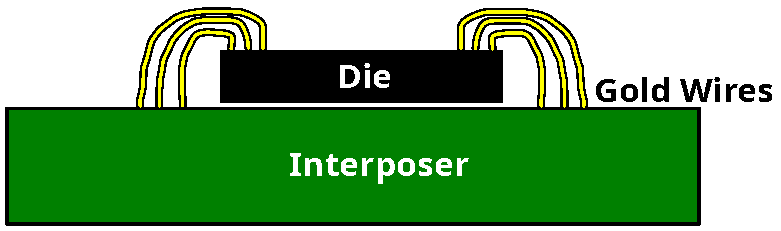
\includegraphics[width=0.8\linewidth]{figures/wirebond2.pdf}
        \caption{}
    \end{subfigure}
    \hfill
    \begin{subfigure}[t]{0.49\linewidth}
        \centering
        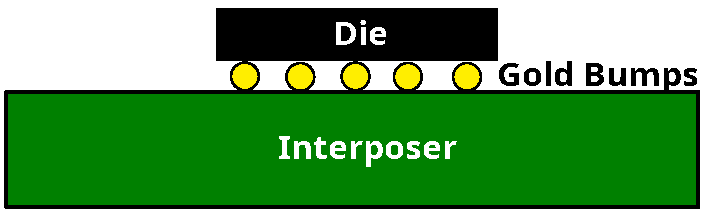
\includegraphics[width=0.8\linewidth]{figures/flipchip2.pdf}
        \caption{}
    \end{subfigure}
    \caption{Comparison of integrated circuit interconnection approaches: (a) wire bonding and (b) flip-chip bonding.}
    \label{fig:flipchip_vs_wirebond}
\end{figure}

State-of-the-art demonstrators typically rely on multilayer ceramic or silicon carriers, combined with solder-based controlled-collapse chip connection (C4) bumps. Although these stacks deliver excellent RF performance, they require expensive thin-film processing and dedicated bumping lines. Glass substrates have emerged as an attractive alternative due to their low permittivity, panel-level scalability, and a custom-made thermal expansion coefficient (CTE)~\cite{Keech2013}. Thermosonic (TS) gold stud bumps offer a solder-free option that avoids under-bump metallurgy and reflow cycles. Recent works have optimized the bump distribution for TS bonding~\cite{Chang2022}, proposed high-reliability Au–Au pad designs~\cite{Yan2024}, and demonstrated Au bump flip-chip assemblies that operate up to \SI{600}{\celsius} in Stacking integrated Circuits (SiC)~\cite{Li2024}. However, limited studies focus on RF characterizations of Au bumps on single-layer glass interposers and on quantitative yield analysis of this integration approach.

In this work we propose a simple and fully in-house integration flow that combines a glass interposer patterned with a single \SI{50}{\nano\metre}/\SI{100}{\nano\metre} Ti/Au metal layer, and \SI{70}{\micro\metre}-wide thermosonic (TS) Au bumps placed using a standard wire-bonding machine. Both the bump placement and the subsequent flip-chip bonding via thermo-compression are performed entirely outside of a cleanroom environment. The electrical behaviour over frequency of individual Au bump interconnections on glass has been experimentally characterized. The captured data has been further fitted to a low-frequency lumped model, enabling accurate prediction of interconnect parasitics in the assembled system over the frequency range between \SI{10}{\mega\hertz} and \SI{10}{\giga\hertz}.

% Structure
The rest of the paper is organized as follows: Section~\ref{sec:model} deals with the lumped-element model of the interconnection bumps and the coplanar waveguides (CPW) on the interposer. Section~\ref{sec:fabrication} describes the bump formation, flip-chip bonding, and sample inspection. Section~\ref{sec:results} focuses on the experimental results, and Section~\ref{sec:results} concludes the study.

\section{Modeling and Interposer Design}\label{sec:model}
To evaluate the electrical performance of the proposed integration flow, a Gallium nitride (GaN) transceiver front-end (TXFE) chip is selected as a test vehicle. The GaN TXFE chip is flip-chip bonded using thermosonic Au bumps onto a single-layer glass interposer featuring ground-signal-ground (GSG) RF connections. The GSG configuration enables the indirect characterization of the bump–line interconnect structure through deembedding of S-parameter measurements.

\subsection{Bump--Line Model Simulation}\label{subsec:bump_line_model}

Each RF connection between the die interposer consists of three thermosonically bonded Au bumps. The CPWs integrated on the interposer are shown on the top and bottom of Fig.~\ref{fig:interposer}(a). This connection is modeled as a concatenation of lumped-elements representing the GSG coplanar waveguide and thermosonic Au bumps, followed by the TXFE die, as illustrated in Fig.~\ref{fig:lumped_element_model}.
\begin{figure}[htbp]
    \centering
    \begin{subfigure}[t]{0.32\linewidth}
        \centering
        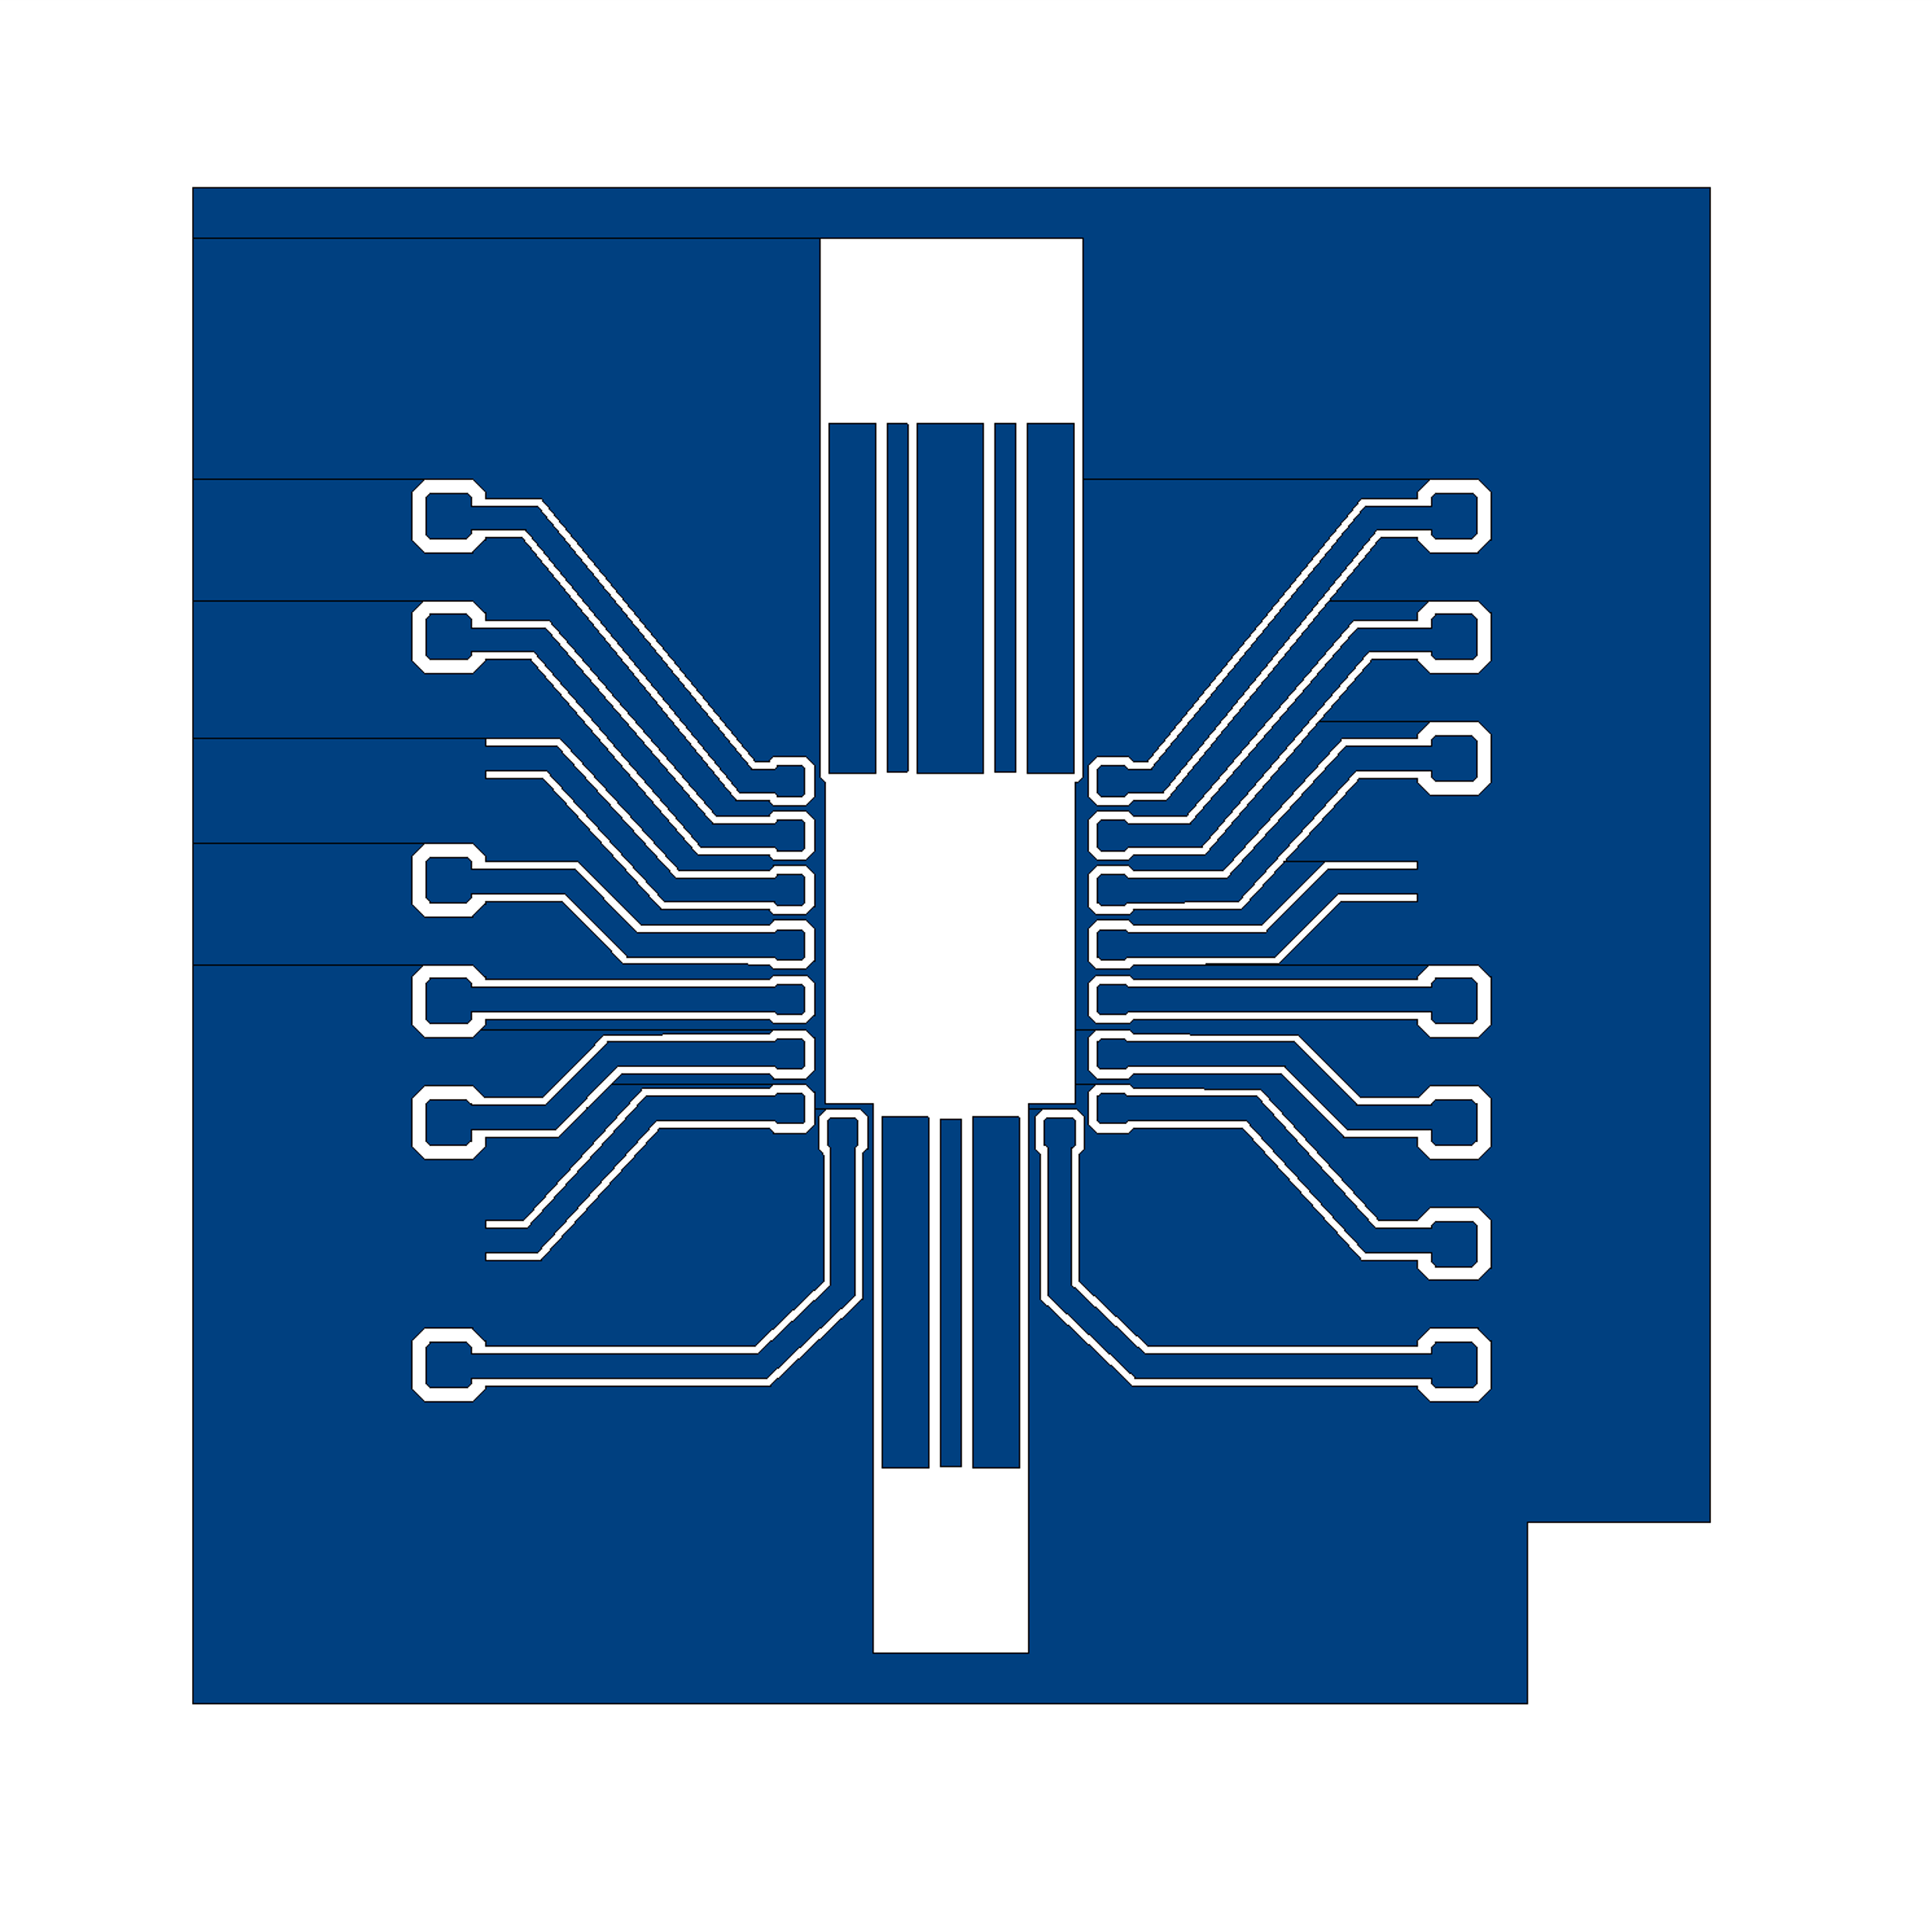
\includegraphics[width=\linewidth]{figures/Interposer_mask_sq.png}
        \caption{}
        \label{fig:interposer_mask}
    \end{subfigure}
    \hfill
    \begin{subfigure}[t]{0.32\linewidth}
        \centering
        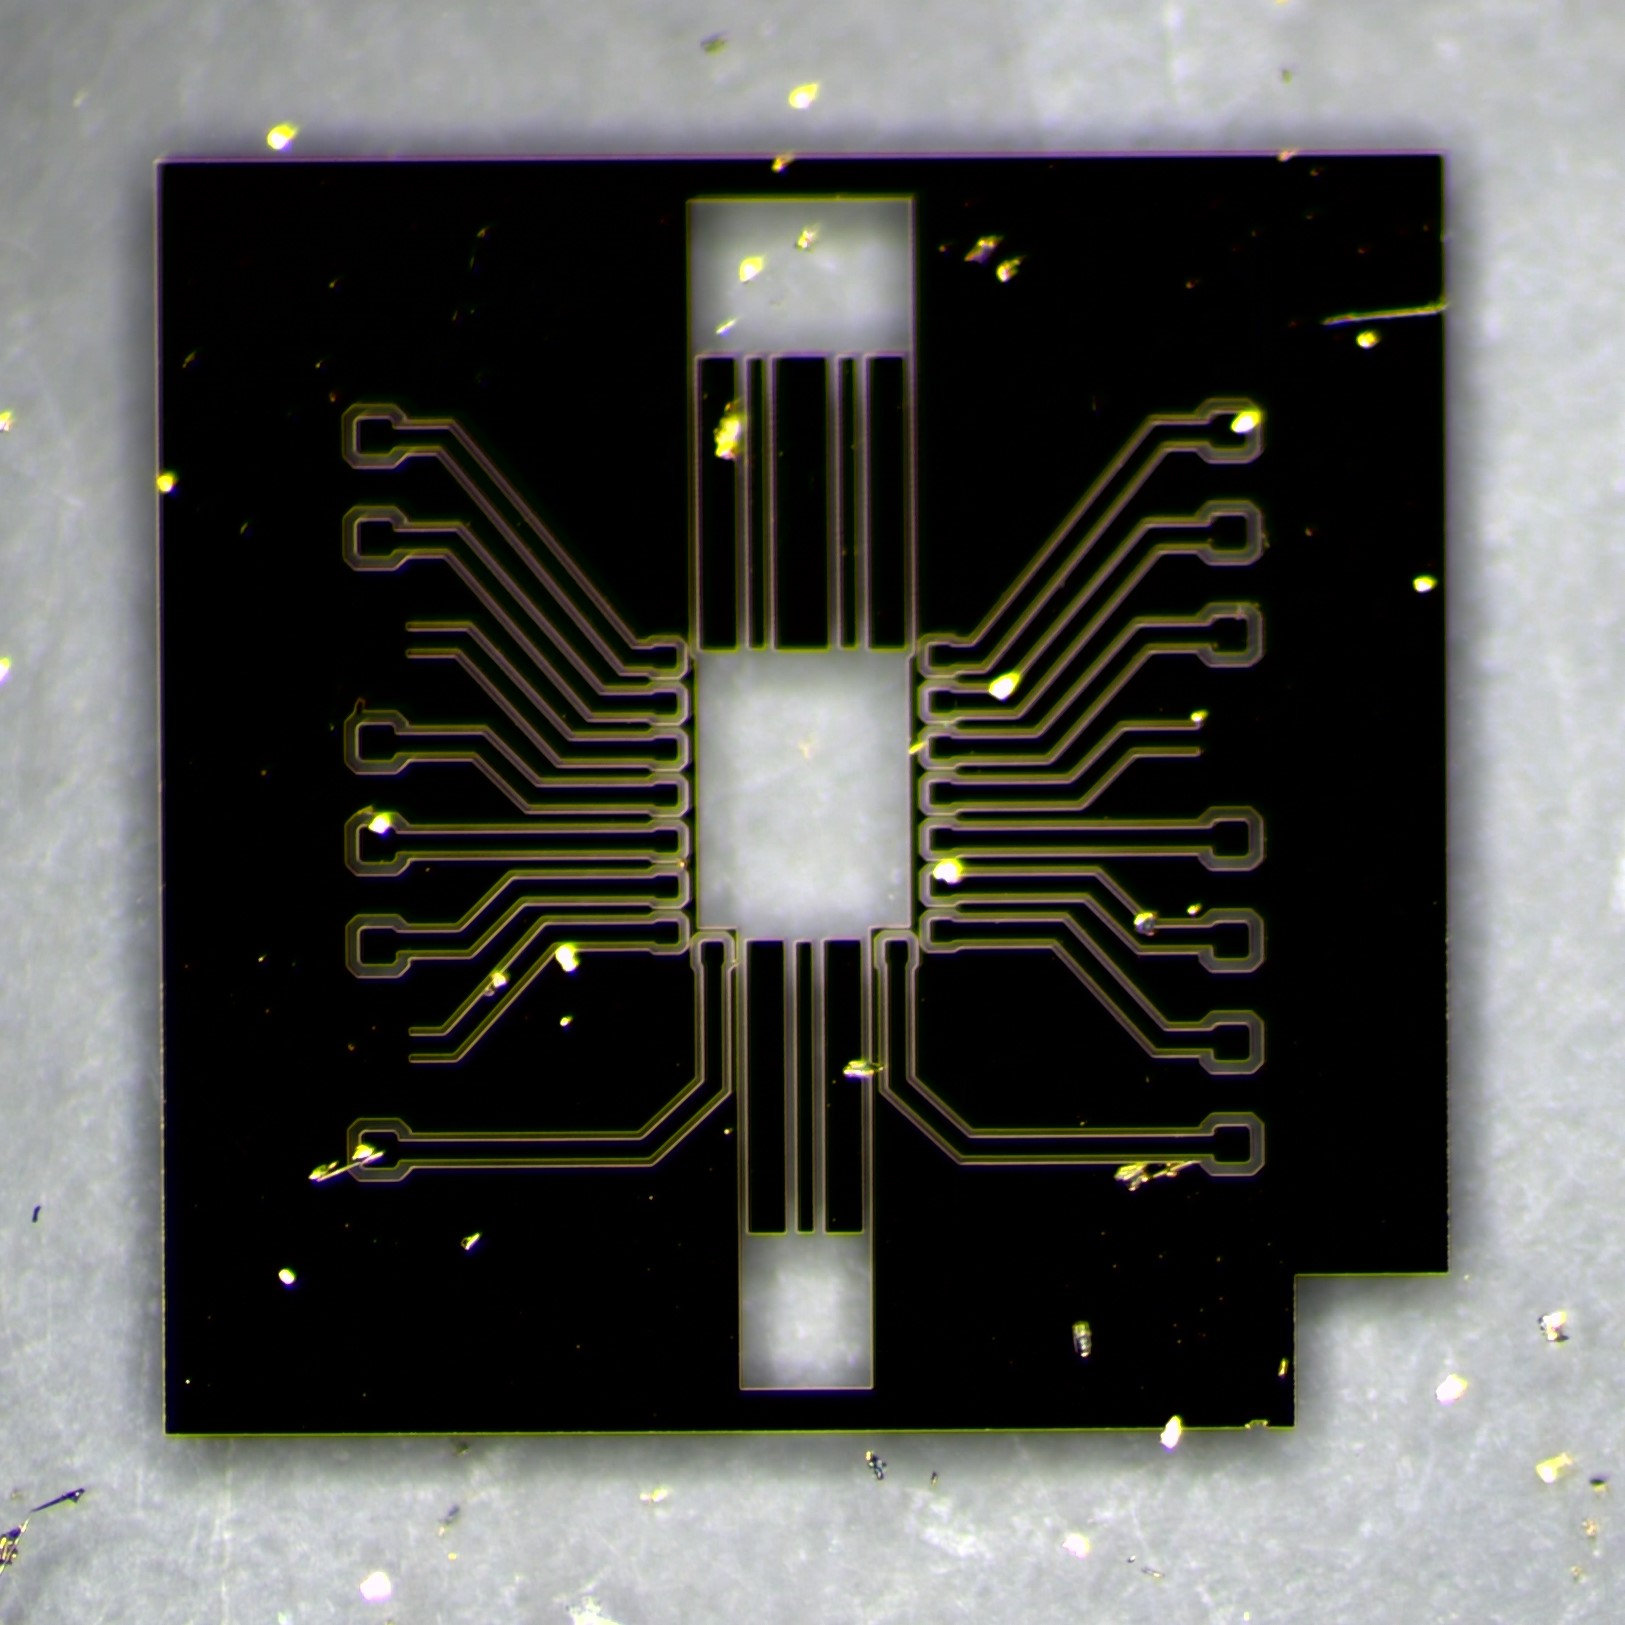
\includegraphics[width=\linewidth]{figures/Interposer_micrograph_sq.jpg}
        \caption{}
        \label{fig:interposer_micrograph}
    \end{subfigure}
    \hfill
    \begin{subfigure}[t]{0.32\linewidth}
        \centering
        \includegraphics[width=\linewidth]{figures/Interposer_flipped_sq.png}
        \caption{}
        \label{fig:interposer_flipped}
    \end{subfigure}
    \caption{(a) interposer digital mask, (b) fabricated interposer and (c) micrograph of the flip-chip bonded die on interposer.}
    \label{fig:interposer}
\end{figure}
%
\begin{figure}[htbp]
    \centering
    \resizebox{\linewidth}{!}{%
        \begin{circuitikz}[american voltages]
            % circuit
            \draw (0,-2)
            node[tlground]{}
            -- ++ (0,0.5)
            to [V, invert] ++(0,1)
            to [R, l = \SI{50}{\ohm}, resistors/scale=0.75] ++ (0,1)
            |- ++ (1,0.5)
            to [R=$R_{\text{CPW}}$] ++(1.5,0)
            to [L=$L_{\text{CPW}}$] ++ (1.5,0) coordinate(bb1)
            -- ++(0.25,0)
            to [R, l_=$G_{\text{CPW}}$, *-] ++(0,-2)
            node[tlground]{};
            \draw (bb1)
            -- ++(1,0) coordinate(bb2)
            to [C=$C_{\text{CPW}}$, *-] ++ (0,-2)
            node[tlground]{};
            \draw (bb2)
            -- ++(2.5,0) coordinate(bb3)
            -- ++ (0.25,0)
            to [R=$\tfrac{3}{2}R_{\text{b}}$] ++ (1.5,0)
            to [L=$\tfrac{3}{2}L_{\text{b}}$] ++(1.5,0) 
            -- ++(0.75,0)
            to [twoport, t=\small TXFE] ++ (0,-3)
            node[tlground]{};
            \draw (bb3)
            to [C=$2C_{\text{b}}$, *-] ++ (0,-2)
            node[tlground]{};
    
            % boxes
            \draw[dashed] (0.75,1.75) rectangle (6.5,-1.25);
            \node[below] at (3.625,2.25) {Ti/Au GSG CPW};
            \draw[dashed] (6.75,1.75) rectangle (10.75,-1.25);
            \node[below] at (8.75,2.25) {3 Au bumps};
        \end{circuitikz}
        }
        \caption{One-port schematic used for characterization, consisting of the CPW transmission line, three-bump transition, and the measured 1-port S-parameters of the TXFE die. }
    \label{fig:lumped_element_model}
\end{figure}
%
The GSG CPW on the interposer has a signal strip width $w$, and signal-ground gap width $s$, of \SI{69}{\micro\meter} and \SI{41}{\micro\meter} respectively. From this, the model parameters can be determined using~\cite{Simons2004}
%
\begin{align}
    R'&=\frac{\rho}{wt}= \SI{4.82}{\ohm / \milli\meter},\\
    C'&=\frac{\sqrt{\varepsilon_{\text{eff}}}}{Z_{0}c}= \SI{111}{\femto\farad / \milli\meter},\\
    L'&=Z_{0}^{2}C' = \SI{437}{\pico\henry / \milli\meter},\\
    G'&=\omega C'\tan\delta= \SI{5.56}{ \nano S/\milli\meter} \;\;(@\SI{10}{\mega\hertz}),
\end{align}
%
Which, when multiplied by the physical length of the GSG traces $l=\SI{1.15}{\milli\metre}$, yield the parameters $R=\SI{5.54}{\ohm}$, $L=\SI{503}{\pico\henry}$, $C=\SI{128}{\femto\farad}$, and $G = \SI{6.39}{\nano S}$. Only the resistance of the gold layer is considered, due to the higher resistivity of the parallel titanium layer. Comparable impedance values for single-metal glass interposers have been reported in~\cite{Wang2016}.

Each gold stud bump is formed by coining a \SI{25}{\micro\meter} gold wire into a nominal bump with diameter $D_b = \SI{70}{\micro\meter}$, radius $r_b=\SI{35}{\micro\meter}$, and height $h_b = \SI{25}{\micro\meter}$. The lumped-element parameters of a single bump are estimated using ~\cite{Simons2004, Grover2009,Paul1994}, leading to:
\begin{align}
    R_{\text{b}}&=\frac{\rho h_{\text{b}}}{\pi r_{\text{b}}^{2}}=\SI{324}{\micro\ohm},\\
    L_{\text{b}}&=\mu_{0}h_{\text{b}}\left[\ln\left(\frac{4h_{\text{b}}}{r_{\text{b}}}\right)+1\right]=\SI{64.4}{\pico\henry},\\
    C_{\text{b}}&=\frac{\varepsilon_{0}\varepsilon_{\text{eff}}\pi r_{\text{b}}^{2}}{s} =\SI{3.64}{\femto\farad}.
\end{align}
%
The lumped-element models offer a compact and predictive representation of the bump–line interconnect structure. With the modeling framework in place, the next section details the physical implementation of the interposer and bump structures.

\section{Flip Chip Bonding Process and Measurement}\label{sec:fabrication}
The interposer is fabricated using a contact photolithography with a film photomask and a negative photoresist. A \SI{50}{\nano\meter}/\SI{100}{\nano\meter} Ti/Au metal stack is evaporated onto the patterned resist, followed by lift-off to form the conductive traces.

\subsection{Gold Bump Placement}\label{subsec:gold_bump}
The gold bumps were deposited using a TPT HB16 thermosonic bonder with \SI{25}{\micro\metre} gold wire. The bonding parameters, summarized in Table~\ref {tab:bump_param}, follow the framework recommendations presented in \cite{Jordan2002} and are optimized for the Ti/Au stack on glass. Heating the interposer at \SI{150}{\celsius} minimizes the tear-off of the Au pad, but provides sufficient temperature for round stud bump formation. Optical inspection confirms coined bump diameters of $D_b =$ \SIrange{65}{75}{\micro\meter}, minimized pad tear-off, and reduced bump tail formation.

\begin{table}[htbp]
    \caption{Proposed TPT HB16 bump formation profile} \label{tab:bump_param}
    \centering
    \begin{tabular}{|l|c|}
        \hline
        \textbf{Parameter}  & \textbf{Value} \\ \hline
        Chuck temperature   & \SI{150}{\celsius} \\
        1st bond force      & \SI{250}{mN} \\
        1st US power        & \SI{120}{mW} \\
        1st US time         & \SI{500}{ms} \\
        2nd bond force      & \SI{35}{mN} \\
        2nd US power        & \SI{60}{mW} \\
        2nd US time         & \SI{60}{ms} \\
        Tail step           & \SI{100}{\micro\metre}\(\times4\)\\
        Up-CO height        & \SI{300}{\micro\metre} \\ \hline
    \end{tabular}
\end{table}

\subsection{Flip-Chip Die-to-Interposer Bonding}\label{subsec:flipchip}
Flip-chip bonding was carried out with the Dr. Tretsky T-5300. A
placement force of \SI{20}{g} per bump was selected after that yield trials revealed
die slippage at \SI{35}{g} per bump.  For \(D_b=\SI{70}{\micro\metre}\), the resulting bump pressure is \SI{51.0}{\MPa}, well above the \SI{1}{MPa} minimum generally recommended for Au-Au thermocompression bonds on the Finetech platform~\cite{Deng2016}. The six-step heat profile provided in Table~\ref{tab:flipchip} has been preferred to a four-step ones, to gradually heat the interposer. The stabilization stage ensures thermal uniformity between the interposer and the heating pad, while the transition from Step 3 to Step 4 provides additional temperature margin for bonding large bumps without oversoftening the Ti/Au pads.

\begin{table}[htbp]
    \caption{Proposed thermo-compression flip-chip bonding profile}
    \label{tab:flipchip}
    \centering
    \begin{tabular}{|l|c|c|c|}
        \hline
        \textbf{Step}          & \textbf{Ramp} (\si{\celsius/s}) & \textbf{Time} (\si{\second}) & \textbf{Target} (\si{\celsius}) \\\hline
        1  (pre-heat)           & 5   & 30 & 90   \\
        2  (pre-heat)            & 10  & 15 & 100  \\
        3  (stabilize)          & 10  & 15 & 250  \\
        4  (touch-down)         & 10  & 5  & 300  \\
        5  (coin)               & 20  & 60 & 350  \\
        6  (cool)               & 10  & 30 & 80   \\\hline
    \end{tabular}
\end{table}

\subsection{S-Parameter characterizations}\label{subsec:vna}
All S-parameter measurements were performed using an MPI THz-Selection probe station equipped with $|Z|$ GSG probes and a Keysight PNA-X N5247B network analyzer, as shown in Fig.~\ref{fig:probe_station}. The measurements covered a frequency range from \SI{10}{\MHz} to \SI{10}{\GHz}.

\begin{figure}[htbp]
    \centering
    \begin{subfigure}[t]{0.59\linewidth}
        \centering
        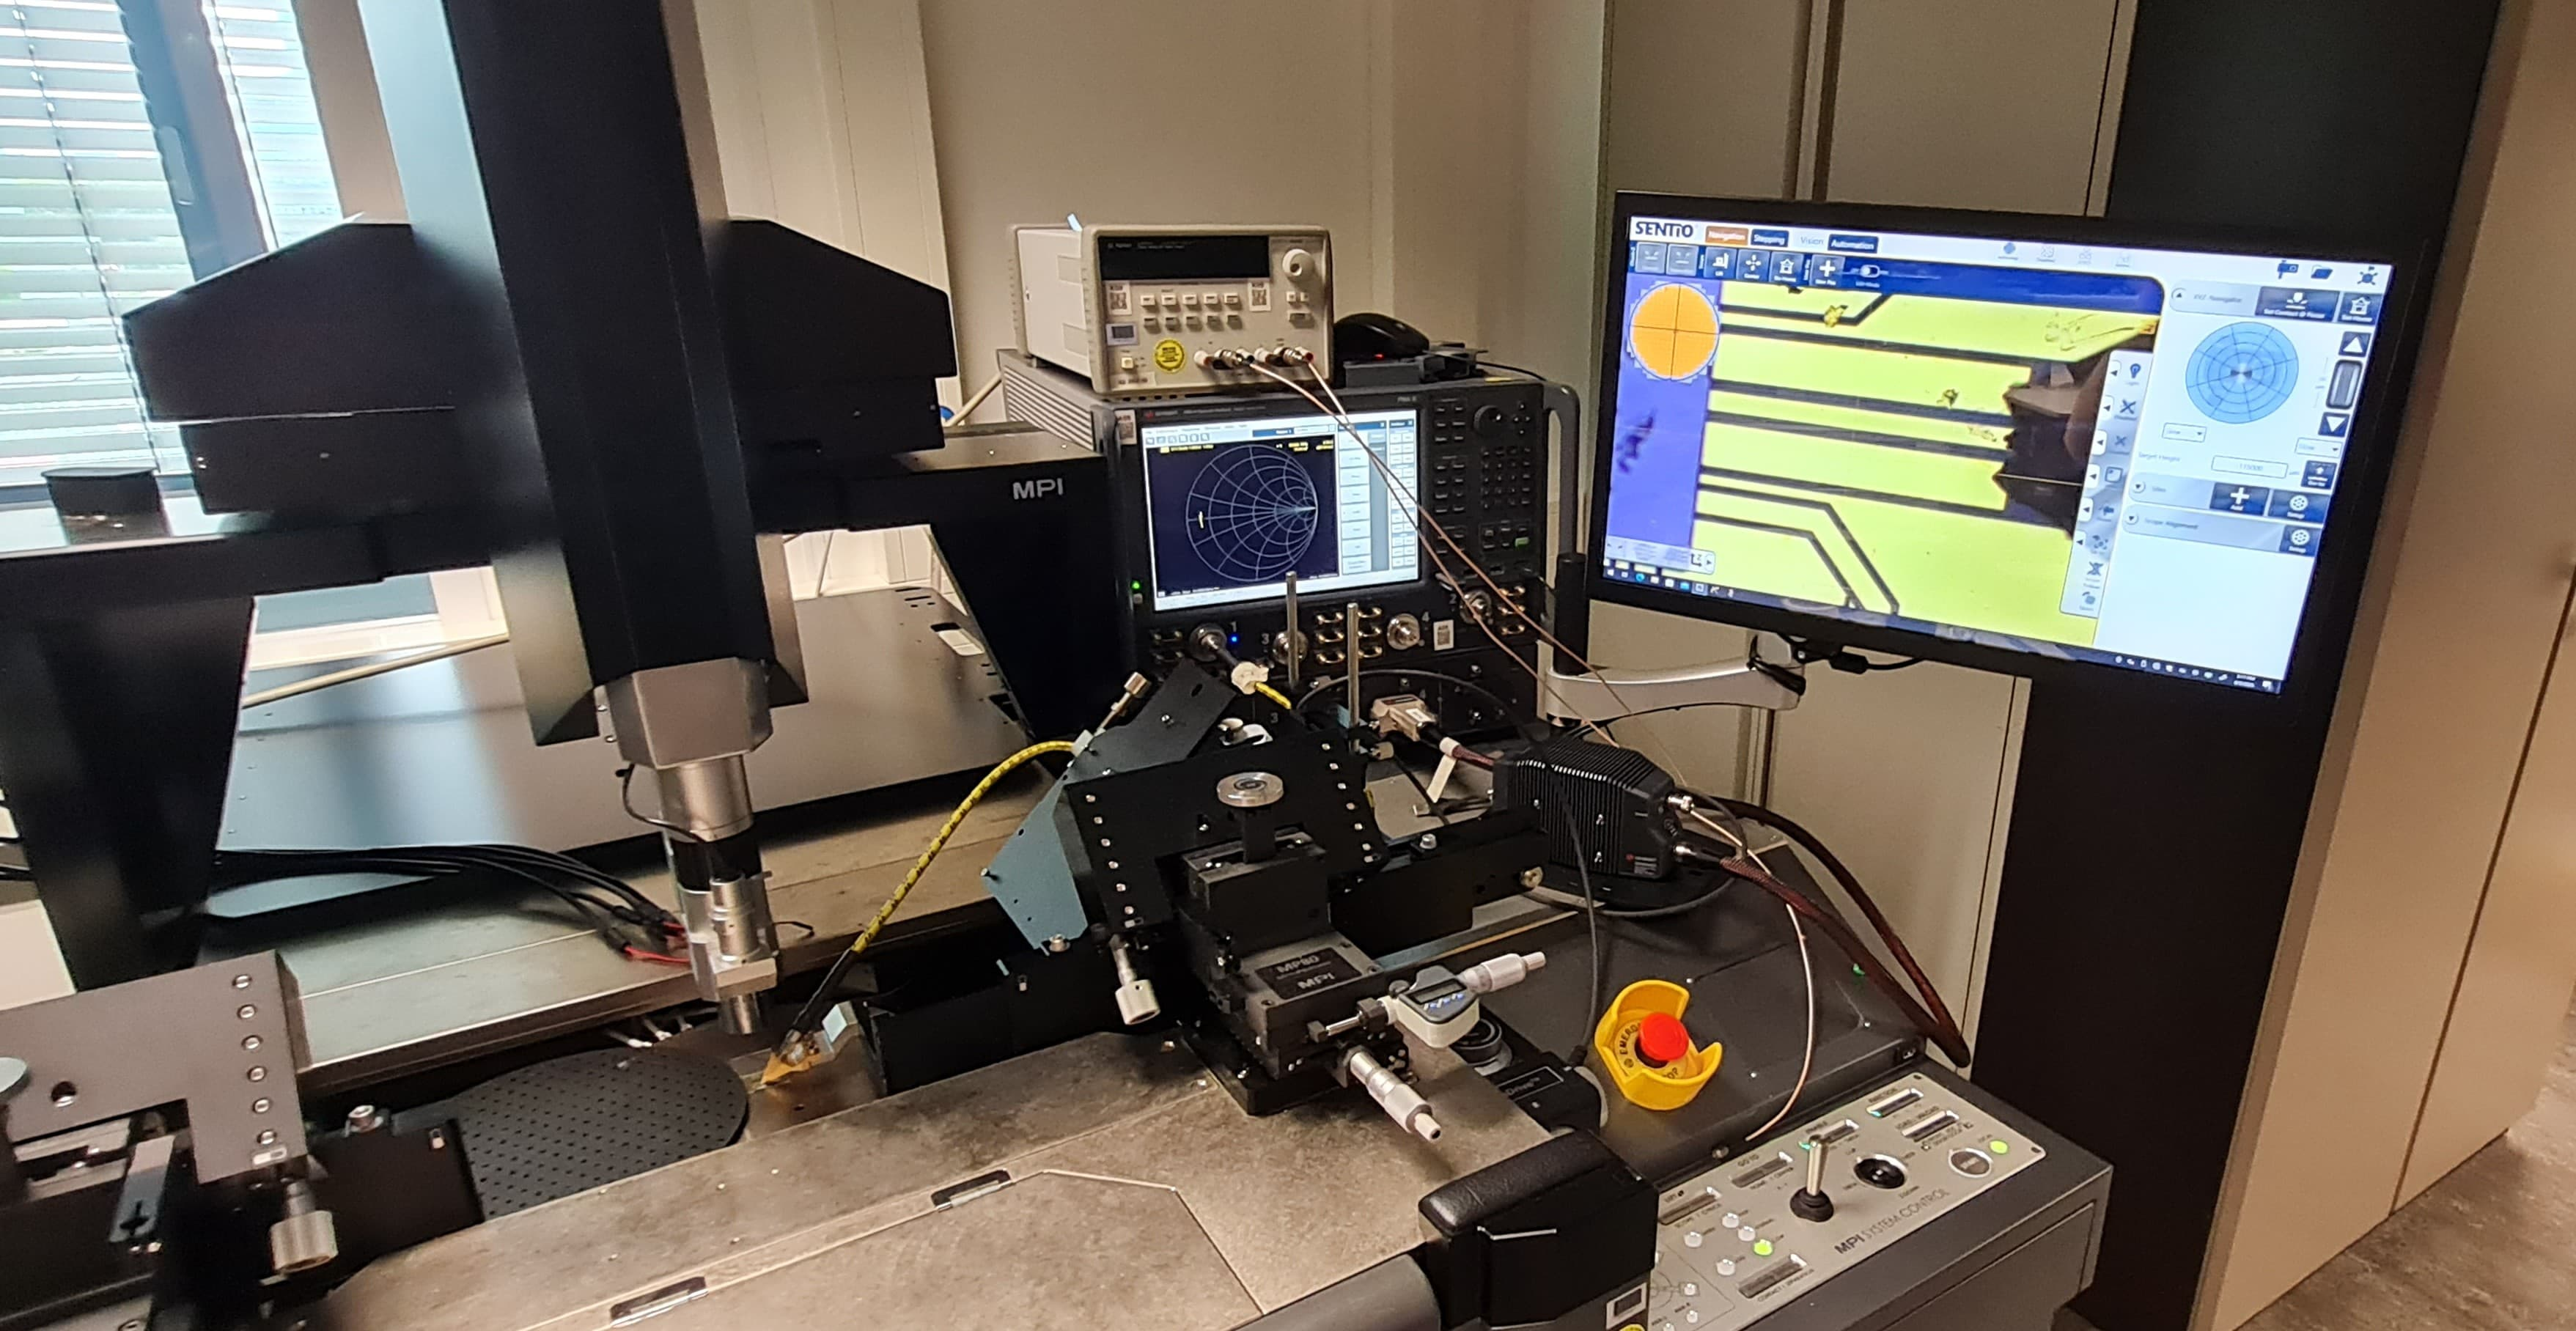
\includegraphics[width=\linewidth]{figures/VNA_machine_setup.jpeg}
        \caption{}
        \label{fig:VNA_setup}
    \end{subfigure}
    \hfill
    \begin{subfigure}[t]{0.39\linewidth}
        \centering
        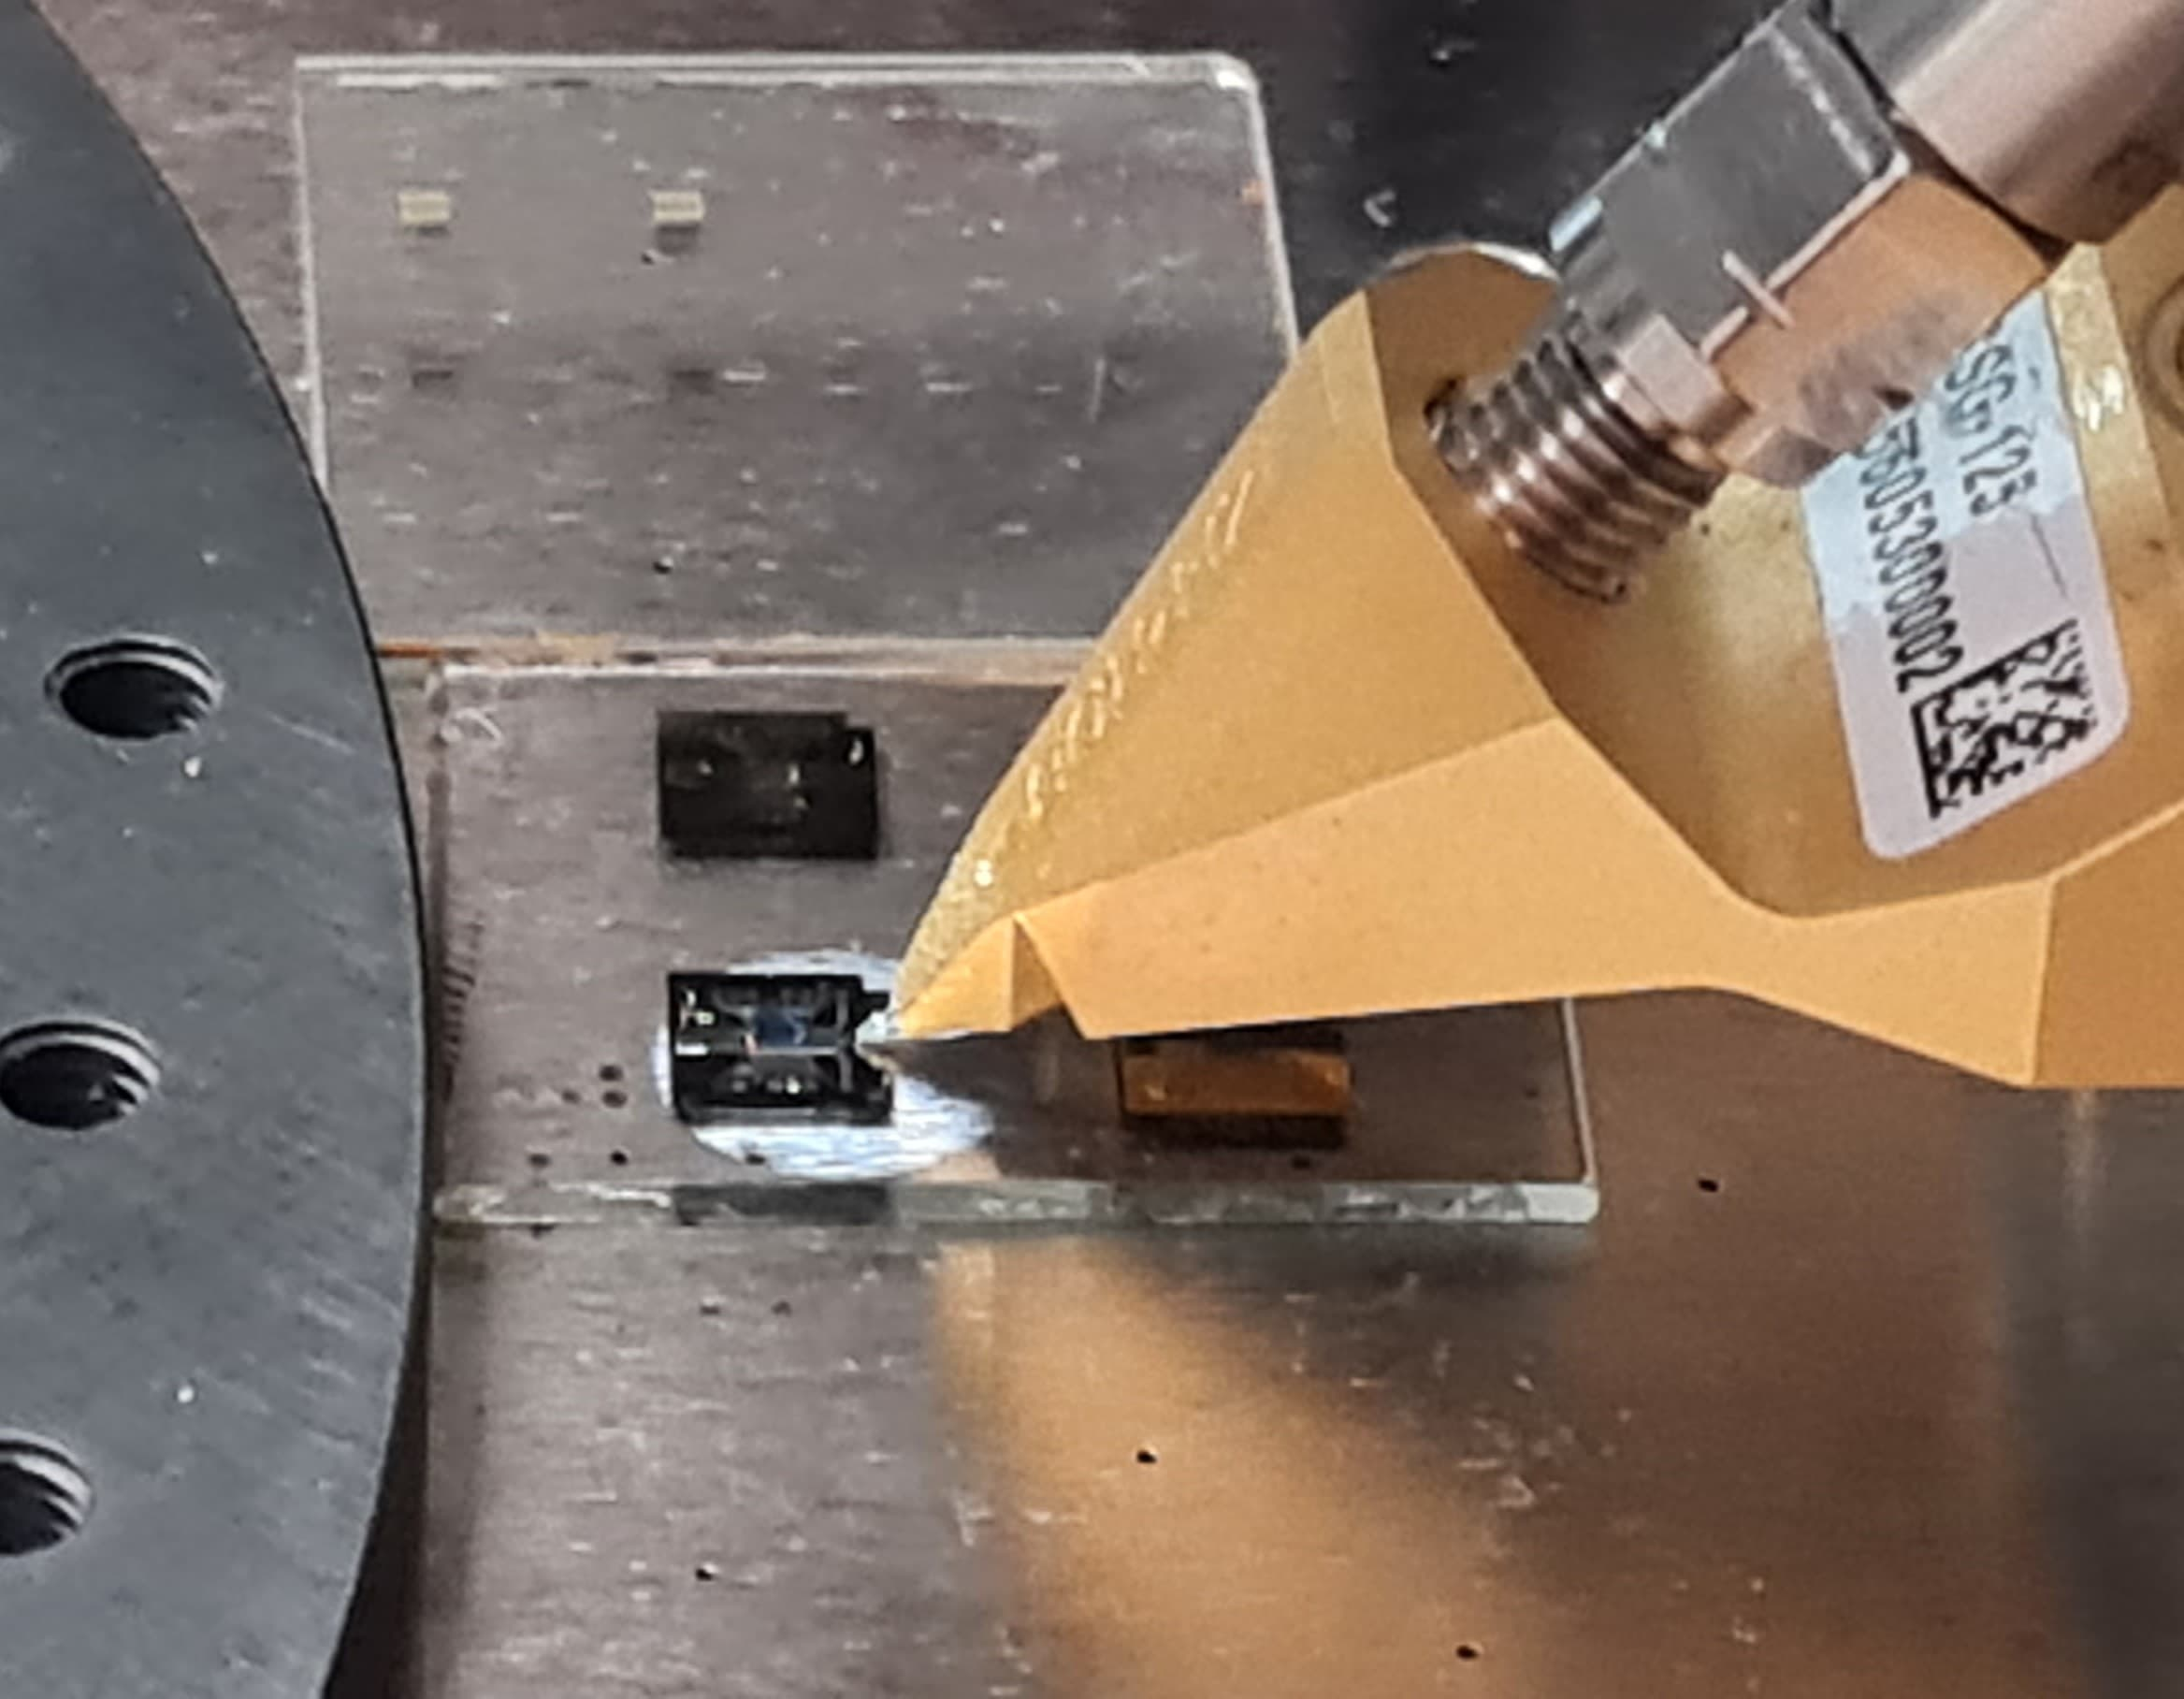
\includegraphics[width=\linewidth]{figures/interposer_probed.jpeg}
        \caption{}
        \label{fig:probe}
    \end{subfigure}
    \caption{(a) MPI THz-Selection probe station setup with the Keysight PNA-X N5247B network analyzer. (b) Close-up of the $|Z|$ GSG probes during direct die measurements.}
    \label{fig:probe_station}
\end{figure}
\section{Results and Discussion}\label{sec:results}
\subsection{Extracted CPW and Interconnection Parameters} \label{subsec:extraction}
A dedicated test structure consisting solely of the coplanar waveguide was fabricated to characterize its intrinsic electrical parameters. This structure isolates the CPW from other circuit elements, enabling extraction of its lumped-element model components. From the short-circuit measurement, the series resistance $R_{\rm{CPW}}$ and inductance $L_{\rm{CPW}}$ were determined to be \SI{6.47}{\ohm} and \SI{119}{\pico\henry}, respectively. Next, the $C_{\rm{CPW}}$ is extracted from the open-circuit measurement to be \SI{94.4}{\femto\farad}. The shunt conductance $G_{\rm{CPW}}$ could not be extracted with sufficient confidence due to its low magnitude relative to the capacitive impedance $Z_C$. This is typical for CPW structures on low-loss substrates, where dielectric losses are negligible and fall below the sensitivity threshold of the measurement setup.

With the CPW characterized, it is possible to deembed its contribution from the measurements of the whole assembly. By performing direct measurements on the die that is flip-chip bonded, the model parameters can be fitted on the measured data. At low frequency, the impedance solely consists of $R_B$, which is extracted to be \SI{3.45}{\ohm}. The fitted capacitance and inductance of the model presented in Fig.~\ref{fig:lumped_element_model}, $C_b$ and $L_b$ are found to be \SI{249}{\femto\farad} and \SI{178}{\pico\henry} respectively. Fig.~\ref{fig:MATLABfit} shows that the derived model slightly overestimates (red line) the measured $S_{11}$ reflection coefficient of the gold bumps and die (blue line).

\begin{figure}[htbp]
    \centering
    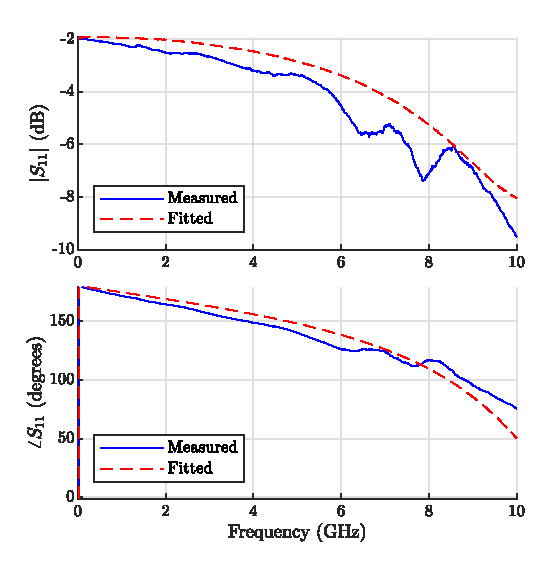
\includegraphics[width=0.8\linewidth]{figures/MATLABfit.eps}
    \caption{Deembedded $S_{11}$ response of the gold bumps and GaN die (blue line), along with the fitted model (red line).}
    \label{fig:MATLABfit}
\end{figure}

By treating the resulting CRL-network as a two-port system, the individual contribution of the bump can be isolated from the surrounding packaging structures. This approach enables the direct calculation of the associated S-parameters, thereby providing a compact yet accurate description of the bump’s behavior that is suitable for integration into system-level simulations.

\begin{figure}[htbp]
    \centering
    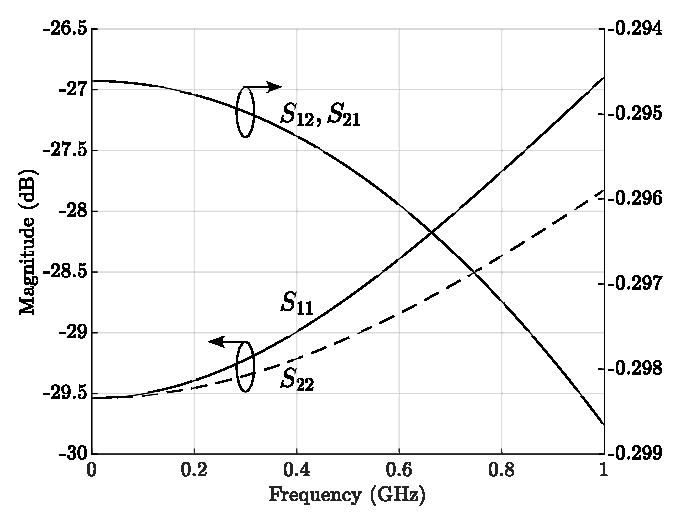
\includegraphics[width=0.8\linewidth]{figures/Sparameter.eps}
    \caption{Measured S-parameter response of a single gold bump, modeled as in Fig.~\ref{fig:lumped_element_model} using parameters extracted from experimental data.}
    \label{fig:model_sparams}
\end{figure}

\subsection{Yield Analysis}\label{subsec:yield_res}
The test structure used for yield validation is shown in Fig.~\ref{fig:yield}. A small interposer was flip-chip bonded onto a larger interposer. Both interposers contain lines and pads, enabling a continuity test to assess how many of the 22 lines can be successfully bonded. Visual inspection and ohmic probing revealed three open circuits, two shorts, and one deformed bump that caused a short during the flip-chip process. Treating these defects as rare events and modeling them using a Poisson distribution, the resulting yield is calculated to be \SI{84}{\percent}.

\begin{figure}[htbp]
    \centering
    \begin{subfigure}[t]{0.49\linewidth}
        \centering
        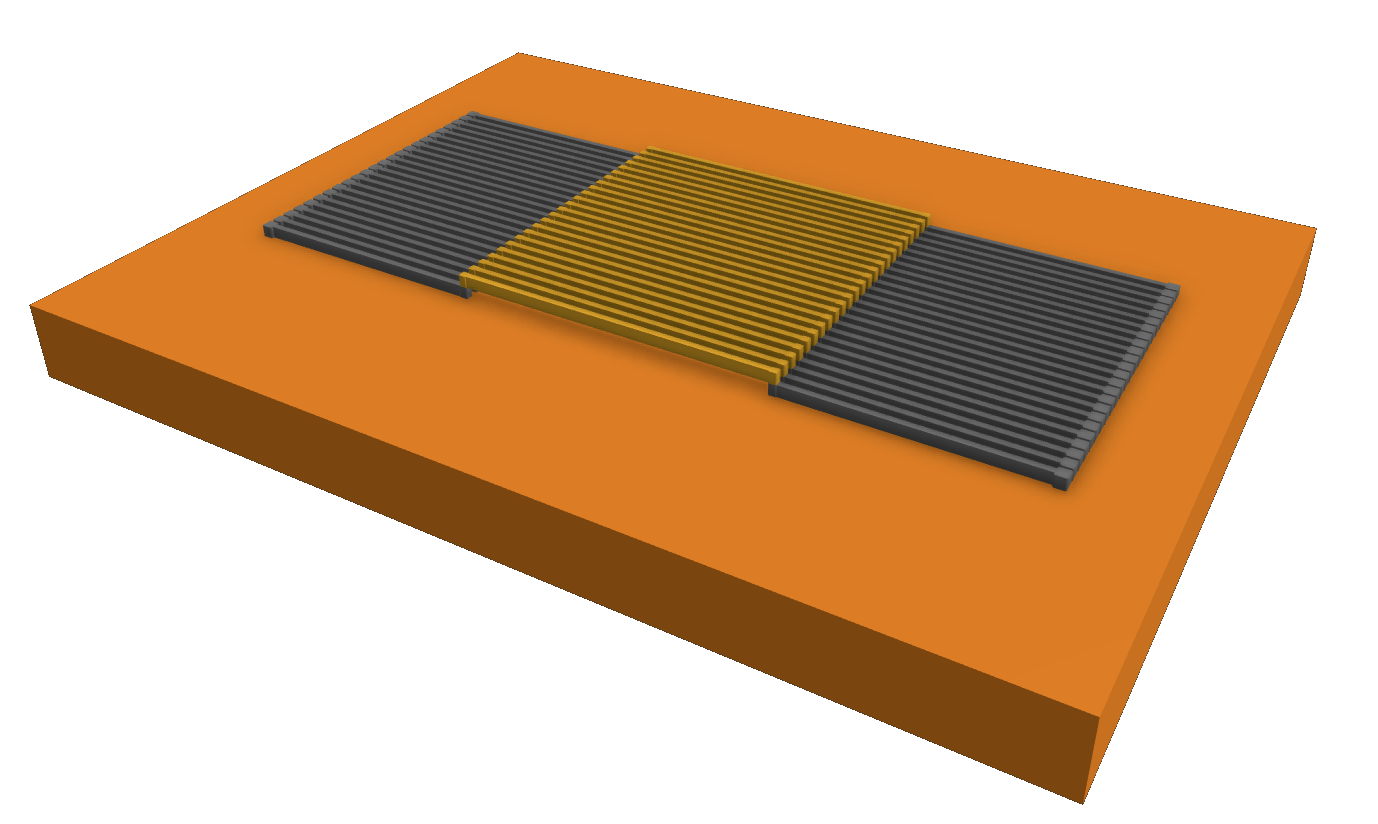
\includegraphics[width=\linewidth]{figures/yield_test_connectors_white.png}
        \caption{}
        \label{fig:yield_render}
    \end{subfigure}
    \hfill
    \begin{subfigure}[t]{0.49\linewidth}
        \centering
        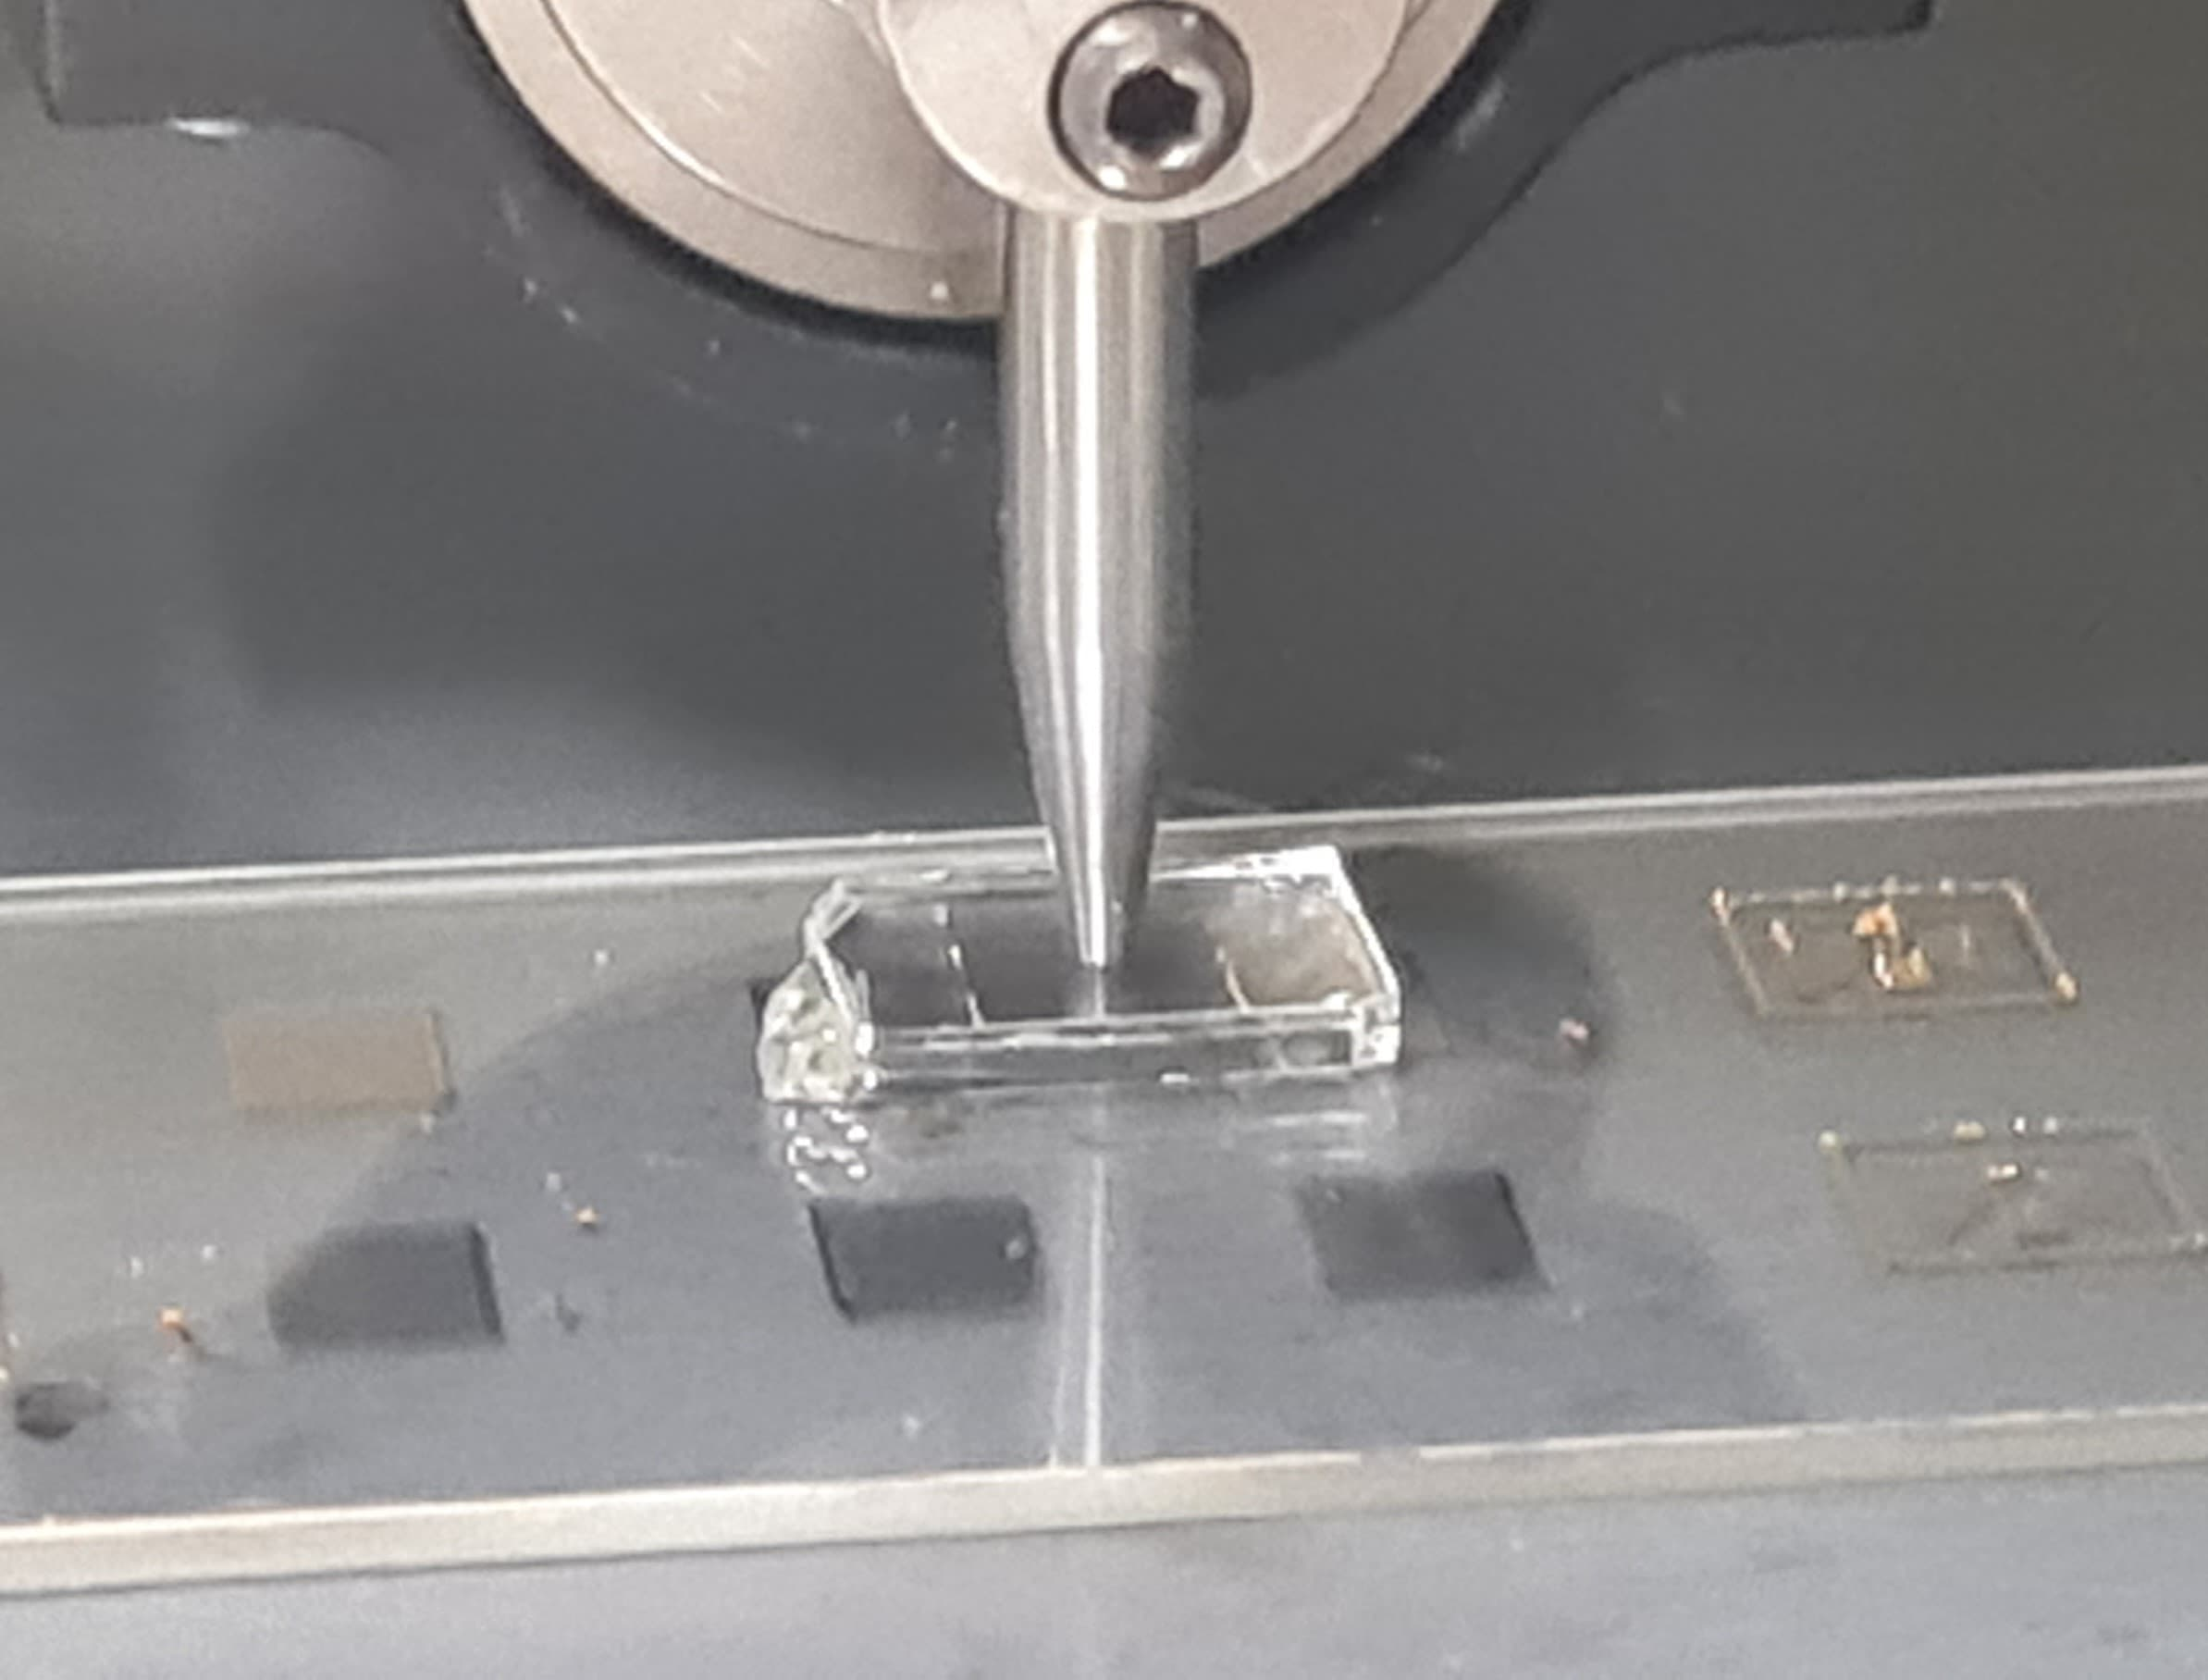
\includegraphics[width=\linewidth]{figures/flip_chipping_fake_die.jpeg}
        \caption{}
        \label{fig:yield_picture}
    \end{subfigure}
    \caption{Yield test structure (a) rendering (top substrate not shown) and (b) flip-chip bonding.}
    \label{fig:yield}
\end{figure}

\subsection{Discussion}\label{subsec:comparison}
Although the single-metal Ti/Au glass interposer with \SI{70}{\micro\metre} Au bumps achieves predictable \SI{10}{\mega\hertz}–\SI{10}{\giga\hertz} performance and an 84\% yield, further validation and research effort are required.

The bump diameters achieved with the current process are comparable to those reported for alternative bumping techniques, as summarized in Table~\ref{tab:integration_comparison}. The process also produced inductance values on the same order of magnitude as other methods, all of which are lower than those associated with wire bonding. However, elevated contact resistance was observed in certain cases, primarily due to poor interposer cleanliness resulting from improper interposer storage conditions. This contamination led to unreliable electrical connections. Yield is expected to improve by developing a suitable interposer cleaning procedures, operating in clean room environments and by improving the accuracy in the placement of the gold bumps. Future process refinements will therefore focus on improving interposer handling and storage to reduce contamination and contact resistance. These improvements aim to establish a more robust and scalable integration method for high-frequency interconnects.

\begin{table}[htbp]
\caption{Comparison of integration approaches for RF chip packaging}
\label{tab:integration_comparison}
\centering
\resizebox{\linewidth}{!}{\begin{tabular}{|l|c|c|c|c|c|}
\hline
& \textbf{This work} % Au bump
& \textbf{\cite{Ullan2006}} % Au bump
& \textbf{\cite{Wright2006}} % C4 bump
& \textbf{\cite{Skup2009}} % Solder bump
& \textbf{\cite{Craninckx1998}} % wire bond
\\ \hline
Type & Au bump & Ball bump & PbSn C4 & Solder bump & Wire bond  \\ \hline
Substr. & \begin{tabular}[c]{@{}c@{}}Ti-Au \\ on glass\end{tabular} & N/A & Silicon & \begin{tabular}[c]{@{}c@{}}Cu-Au \\ on PCB\end{tabular} & \begin{tabular}[c]{@{}c@{}}Al-Cu on \\ CMOS\end{tabular} \\ \hline

$D$ & \SI{75}{\micro\meter} & $<$\SI{55}{\micro\meter} & \SI{25}{\micro\meter} & \SI{150}{\micro\meter} & \SI{25}{\micro\meter} \\ \hline

$R$ & \SI{3.45}{\ohm} & $<$\SI{1}{\ohm} & \SI{10}{\milli\ohm}& \SI{3.7}{\milli\ohm} & $\SI{0.44}{\Omega/\mm}$ \\ \hline

$L$ & \SI{178}{\pH} & N/A & N/A & \SI{50}{\pH} & \SI{1.2}{\pico \henry /\mm} \\ \hline
Yield & 84\% & \SIrange{90}{99.9}{\%} & \SI{99.99}{\%} & N/A & $\approx 100\%$ \\ \hline

\begin{tabular}[c]{@{}l@{}}Proc.\\ comp.\end{tabular} & Low & Outsourced & High & Medium & Low \\ \hline

\end{tabular}}
\end{table}

\section{Conclusion}
A complete process flow for single-layer Ti/Au ground-signal-ground flip-chip interposers on glass substrates has been demonstrated and experimentally validated up to \SI{10}{GHz}. The short-open deembedding of the coplanar waveguide reveals that each \SI{70}{\micro\metre} gold bump can be accurately modeled using a lumped-element representation comprising shunt capacitance, series resistance, and inductance. At \SI{10}{MHz}, the bump behaves predominantly as a \SI{3.4}{\ohm}, at higher frequencies, the \SI{178}{\pH} inductance and \SI{249}{\fF} start to contribute.
Although the fabrication and bonding approach does not match the performance of cleanroom- or solder-based flip-chip processes, it offers a practical and accessible alternative. The method achieves lower inductance compared to conventional wire bonding, thereby improving high-frequency performance.
Yield analysis of a flip-chip bonded small interposer with 22 interconnect lines demonstrated that gold bump placement combined with thermo-compression bonding can achieve a functional yield of \SI{84}{\percent}. These results confirm the viability of the proposed process for prototyping and low-volume integration of high-frequency interposer demonstrators.

% Validated CPWG model
% Bump resistance
% Yield

\section*{Acknowledgment}
The authors would like to thank   Vaggelis Zaoutis, and Eugenio Cantatore for their invaluable support.

\bibliographystyle{IEEEtran}
\bibliography{references}

\end{document}